\documentclass{article}
\usepackage{array}
\usepackage[a4paper, total={6in, 8in}]{geometry}
\usepackage{graphicx}
\newcolumntype{L}[1]{>{\raggedright\let\newline\\\arraybackslash\hspace{0pt}}m{#1}}
\newcolumntype{C}[1]{>{\centering\let\newline\\\arraybackslash\hspace{0pt}}m{#1}}

\begin{document}
\begin{center}
{\huge\textbf {443 Final Project Report}}\\[1in]
{\huge\textbf {ADAMLAR}}\\
\end{center}
\clearpage

{\huge\textbf {1-System Level Structural Diagram}}
\\
\includegraphics[scale=0.8]{System_Level_Structural_Diagram}
\pagebreak
{\huge\textbf {2-Task Decomposition Graph}}
\\
{\huge {Embedded System 1: “Lap Count”}}
\\
\includegraphics[scale=0.2]{Lap_Counter_Task_Decomposition_Graph}
\\[0.2in]
{\huge {Embedded System 2: “Car Control”}}
\\[0.2in]
\includegraphics[scale=0.2]{Speed_Task_Decomposition_Graph}
\clearpage
{\huge\textbf {3-Sequence Diagram}}
\\
{\huge {Embedded System 1: “Lap Count”}}
\\
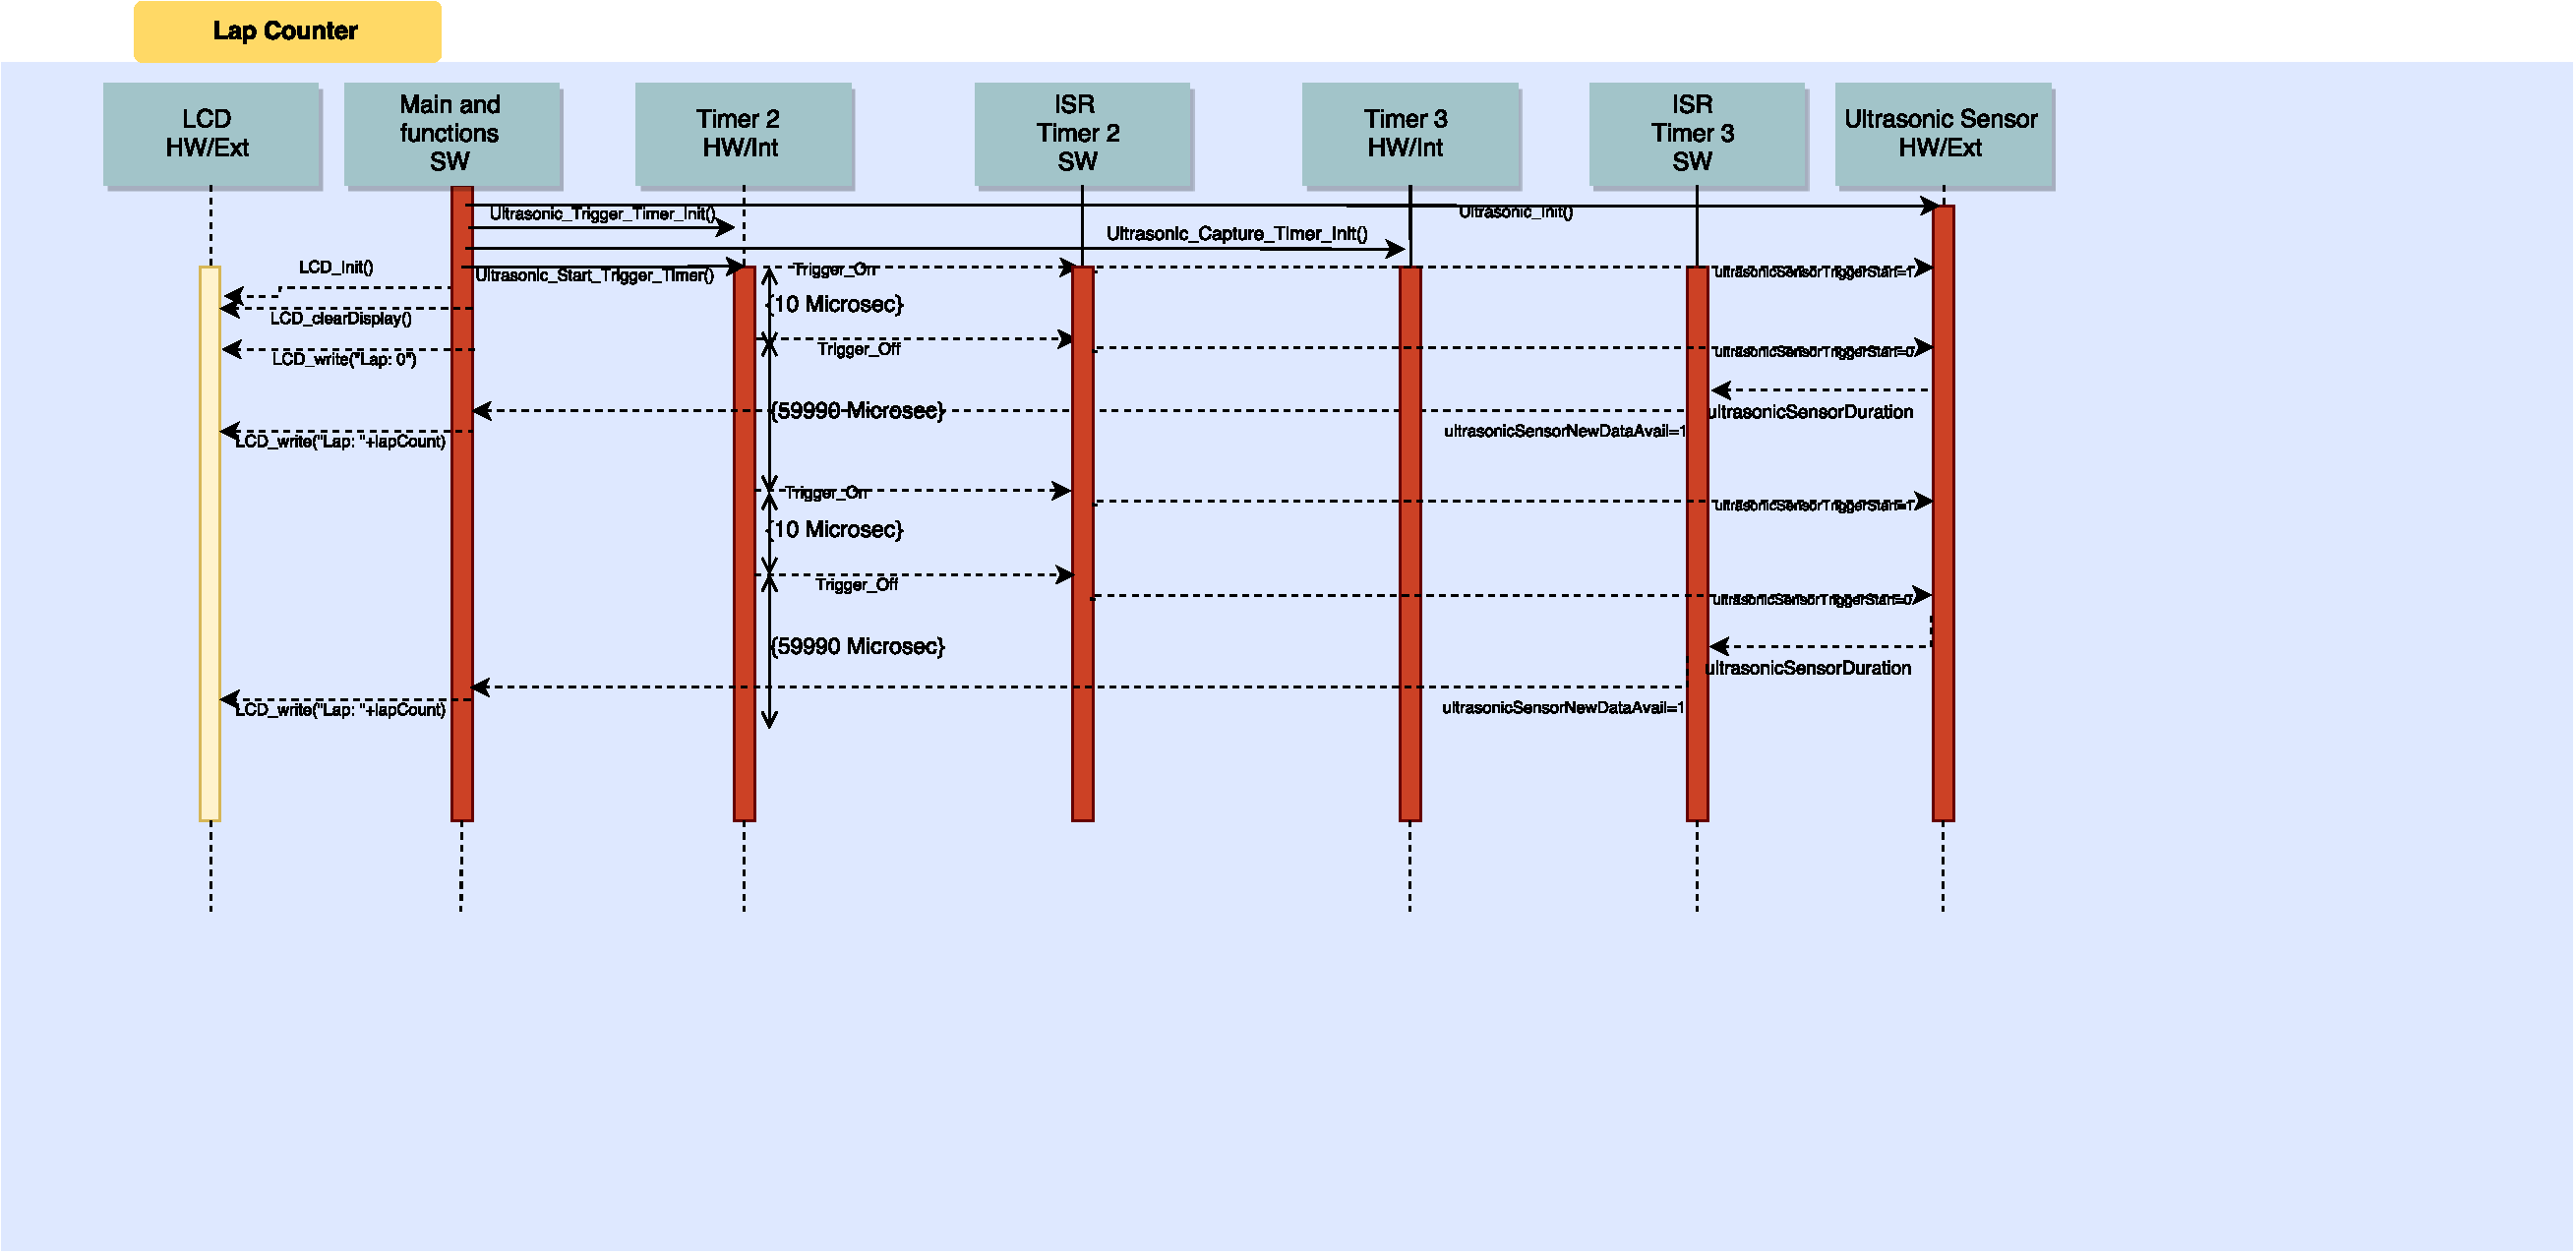
\includegraphics[scale=0.3]{Lap_Counter_Seq_Diagram}
\\
{\huge {Embedded System 2: “Car Control”}}
\\
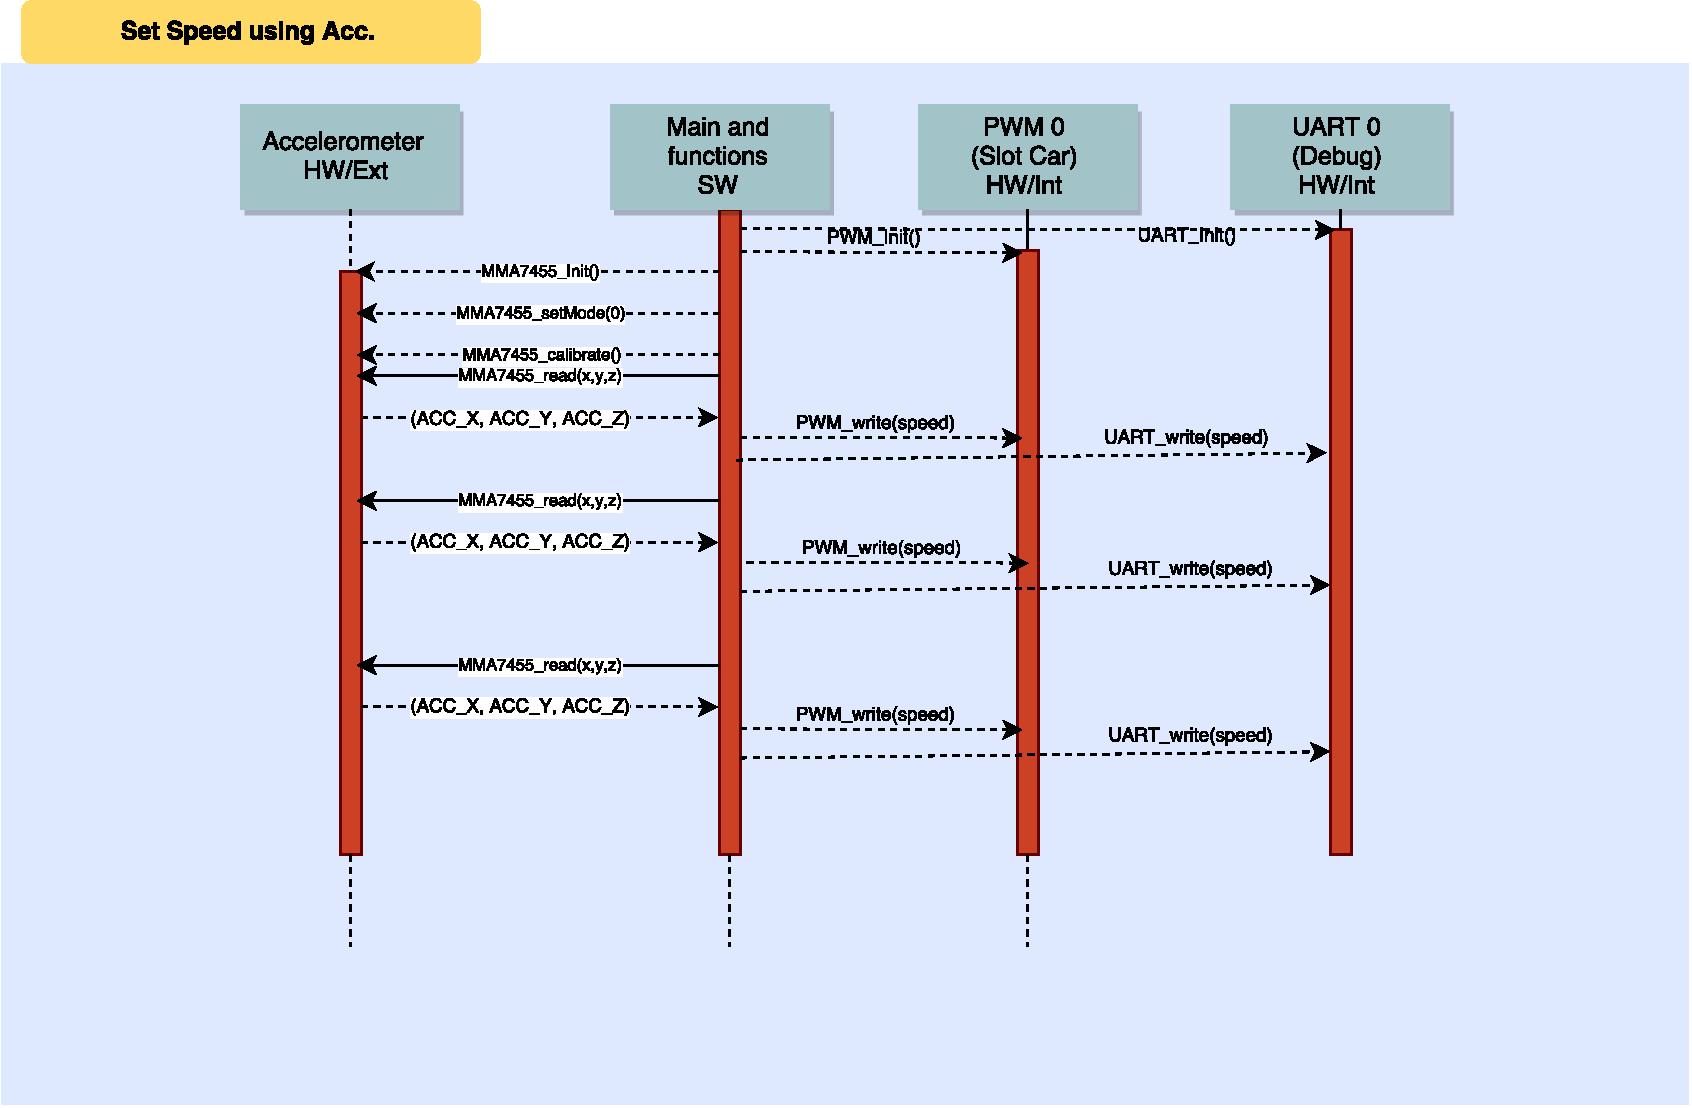
\includegraphics[scale=0.5]{Read_Acc_Control_Speed}
\clearpage
{\huge\textbf {4-Coding}}
\\
{\huge {Embedded System 1: “Lap Count”}}
\\
\begin{tabular}{| C{4cm} | C{4cm} | C{4cm} | C{2cm} |}
\hline
\textbf{Function Name} &\textbf{Function Definition}  & \textbf{Objective} &\textbf{WCET}\linebreak(simulation)\\
\hline
Ultrasonic\_Init() & Initialization of the Ultrasonic sensor. Functions of the trigger
and echo pins connected to the LPC board are defined in the IOCON registers& There are 2 data pins to
communicate with the ultrasonic sensor. Enabling the corresponding pins in the main board, their directions'
(input or output) is set for echo and trigger pins. So that, the board is able to trigger a calculation
of the distance and get the incoming signals with echo pin.& 18 usec\\
\hline
Ultrasonic\_Trigger\_Timer\_Init()&Trigger timer initializer. The output for the trigger pin is
 initialized in this function & Timer 2 is used to synchronize the value(either HIGH or LOW) to the Ultrasonic
 sensor. To initialized it, this function is used. First the power is enabled to this section with PCONP Register
 , then counters (Timer counters and Prescale counters) and match values are set appropriately. Last, the
 function on a match("toggle" in this case) is set. & 31 usec\\
\hline
LCD\_init()&Initialization of the LCD and its pins.& LCD is initialized by setting its pins' functionalities on the board,
and sending correct values to initialize the external driver, ( like 0x03, 0x03,0x03,0x02)&5.18 sec\\
\hline
\end{tabular}
\begin{tabular}{| C{4cm} | C{4cm} | C{4cm} | C{2cm} |}
\hline
Ultrasonic\_Capture\_Timer\_Init()& Echo timer initializer for the echo signal of the ultrasonic sensor.&
First the using PCONP register, the timer is powered on. Then its match registers and timer and prescale timer registers
are given the appropriate functionalities. This timer is used to count the elapsed time from the transmission of the
signals to the echo of the sent signals. So that, the distance of the object could be detected.&21.3 usec\\
\hline
Serial\_init()&Initialization of the UART 0 & Using UART(Serial communication), the debug information of distance of the detected object
and the lap count will be sent to the computer. &57.8 usec\\
\hline
TU()&Task for Ultrasonic, calculates the distance&The distance is calculated detected by ultrasonic sensor.
This distance is used to detect whether the car is in the range or not.&30.6 microsec\\
\hline
TC()& Task for the lap counter & After getting the distance detected, this function checks whether the
distance is smaller than the threshold, if it is, then the lap count is incremented by one. &23.0 microsec\\
\hline
TSD()&Task for system diagnosis, includes sending distance detected and the lap count data from UART
to PC & In order to debug the code, we are using this function which will be printing the value of
distance measured and the lap counted.&192 millisec\\
\hline
TDi()&This function sets the cursor to the appropriate position, then clears the display starting from the
cursor, then writes the lap count into the LCD screen.& To meet the requirements specified,
this function is used. It basically, writes the lap count into the LCD screen.&12.2 microsec\\
\hline
\end{tabular}
{\huge {Embedded System 2: “Car Control”}}
\\
\begin{tabular}{| C{4cm} | C{4cm} | C{4cm} | C{2cm} |}
\hline
\textbf{Function Name} &\textbf{Function Definition}  & \textbf{Objective} &\textbf{WCET}\linebreak(simulation)\\
\hline
TI()&Function initializes all the devices/modules used by the operating code.Basically consists of initializing
accelerometer, PWM pin, &In order to use the devices in the board, we have to initialize them before using.
Powering on the devices(PCONP) and giving the appropriate pin functionalities(IOCON) are done in this step.&5.86 secs\\
\hline
TSS()&Task for setting the speed of the car. To set a speed, first we are reading the angle of the board, from the
accelerometer. Using the angle value of it, the pulse width of the output signal is modulated from 0 to 999 where 500
means that 50\% duty cycle.& To meet the requirements specified, we are using the accelerometer data as input to
set the speed of the slot car. After getting the angle value, the speed of the car is set by using PWM.&44.6 microsec\\
\hline
TGA()&Task for getting the angle of the board using the accelerometer device on it. This function reads the
acceleration data from the device on the LPC board and finds the angle in the X dimension of the device.&
To make the speed of the slot car controllable by an input device, accelerometer device is used and according to
its angle in the X direction, the speed of the car is set. This function realizes the getting the angle data.&79.7 microsec\\
\hline
TSD()&Task for system diagnosis. This function is used to send the speed information to the PC using UART.&To debug the
code that we wrote in this section, the data produced is sent to the PC to oversee the system working.&522 millisec\\
\hline
\end{tabular}
\clearpage
{\huge\textbf {5-Scheduling}}
\\
{\huge {Embedded System 1: “Lap Count”}}
\\
In this part of the project, we are using Polling with interrupts. When a new data
is received using the ISR\_echoCaptureCounter, the flag ultrasonicSensorNewDataAvailable is
set to 1, the pseudo code is as follows:\\
ISR\_echoCaptureCounter()\{\\ if new data then\\ ultrasonicSensorDuration=duration;
ultrasonicSensorNewDataAvailable=1; \\
\}\\
This ISR is initiated after each 60 milliseconds and called when a signal is echoed back to the sensor.
This process of repeated initialization and waiting functions are done via the usage of Timer 2 and Timer 3
together.\\
While the ISR is not running, the main function polls the flag ultrasonicSensorNewDataAvailable.
The execution of the main loop is as follows:\\
while(true)\{\\
TU();//Poll the flag, if there is new data available, then calculate the distance\\
TC();//If the new distance is smaller then the threshold, increment the lap Counter\\
TDI();//Display the lap count value in the LCD\\
TSD();// System diagnosis, send relevant information using UART to debug\\
\}\\
\\
{\huge {Embedded System 2: “Car Control”}}
\\
In this section, there is no interrupt used, the code executes in a cycle and reads data from the
accelerometer. The communication with the accelerometer is done via I2C. An interrupt algorithm could have
been "Set a timer to repeat infinitely with a frequency, check if the value in accelerometer changed and
set a flag if it is changed.". However, this has no benefits over polling the data itself with a frequency,
so we decided that it is more convenient if it is not used. The main schedule of this module program is that:\\
while(true)\{\\
TGA();//Poll the value in accelerometer and calculate angle\\
TSS();//Set the speed of the car using the angle value from acc.\\
TSD();//Send the debug information to the PC\\
\}
\\[0.5in]
\begin{tabular}{| C{4cm} | C{4cm} | C{5cm} |}
\hline
Shared Variable&Name of the function&Name of the ISR\\
\hline
ultrasonicNewDataAvailable&TU& ISR\_echoCaptureCounter\\
\hline
ultrasonicSensorDuration&TU&ISR\_echoCaptureCounter\\
\hline
ultrasonicSensorTriggerStart&TI&ISR\_ultrasonicTriggerToggler\\
\hline
\end{tabular}
\clearpage
{\huge\textbf {6-Timing Diagram}}
\\
\includegraphics[scale=0.5]{Timing_Diagram}
\\
\begin{tabular}{| C{4cm} | C{4cm} | C{1cm} | C{2cm} | C{2cm} |}
\hline
Name of the ISR	 &	Shared Variable				&			Priority&	WCET	&	ACET\\
\hline
ISR\_ultrasonicTriggerToggler &	ultrasonicSensorTriggerStart		&			5	&	6.9 us	&	6.32 us\\
\hline
ISR\_echoCaptureCounter	& ultrasonicSensorDuration, ultrasonicSensorNewDataAvailable&	1	&	8.5 us&		6.1 us\\
\hline
\end{tabular}
\clearpage
{\huge\textbf {7-Hardware Block Diagram}}
\\
\begin{tabular}{| C{4cm} | C{4cm} | C{2cm} | C{2cm} | C{2cm} |}
\hline
Component &Type ID &Quickstart Board & Base-board & Off-board\\
\hline
Ultrasonic  &    HC-SR04  & &&                                             x\\
\hline
LCD       &      LCM-S01601DSR &&&                                         x\\
\hline
Potentiometre &  B10K  &&&                                                 x\\
\hline
Accelerometer &  MMA7455    & &                              X&\\
\hline
LED  &  &  &&                                                              X\\
\hline
1K-Resistor &&&&            X\\
\hline
\end{tabular}
\\[2in]
\begin{tabular}{| C{10cm} | C{2cm} |}
\hline
Expenses& Cost\\
\hline
120pcs 10cm male to male + male to female and female to female jumper wire&\$2.5\\
\hline
\end{tabular}
\clearpage
{\huge\textbf {8-Board Pin Table}}
\\[0.5in]
\begin{tabular}{| C{5cm} | C{5cm} |}
\hline
LCD PINS      &     LPC4088 PINS\\
\hline
1            &         GND\\
\hline
2            &         VU\\
\hline
3        &    to 2. pin of potentiometer\\
\hline
4 RS      &           P0.8 (P12)       \\
\hline
5 RW      &           P0.6 (P14) \\
\hline
6 EN       &          P0.7 (P13)\\
\hline
11 DATA0    &            P0.24 (P16)\\
\hline
12 DATA1     &           P0.25 (P17)\\
\hline
13 DATA2      &          P0.26 (P18)\\
\hline\\
14 DATA3       &         P1.30 (P19)\\
\hline
\end{tabular}
\\[1in]
\begin{tabular}{| C{5cm} | C{5cm} |}
\hline
Potentiometer&LPC4088 PINS\\
\hline
left & Vin\\
\hline
right & GND\\
\hline
\end{tabular}
\\[1in]
\begin{tabular}{| C{5cm} | C{5cm} |}
\hline
Ultrasonic&LPC4088 PINS\\
\hline
Vcc & Vin\\
\hline
GND & GND\\
\hline
Trig Trigger & P0.9(P11)\\
\hline
Echo Echo & P0.23(P15)\\
\hline
\end{tabular}
\\[1in]
\begin{tabular}{| C{5cm} | C{5cm} |}
\hline
Slot Car&LPC4088 PINS\\
\hline
Vcc & P1.5(P28)\\
\hline
GND & GND\\
\hline
\end{tabular}
\\
\clearpage
{\huge\textbf {9-Appendix}}
\\
{\huge {Embedded System 1: “Lap Count”}}\\
\newline
\textbf{main.c}
\begin{lstlisting}
\#include "LPC407x\_8x\_177x\_8x.h"

\#include "Library/Ultrasonic.h"
\#include "Library/SystemStructures.h"
\#include "Library/Timer.h"
\#include "Library/LCD.h"
\#include "Library/Serial.h"
\#include <stdio.h>

int distance = 0 ;
char l = 0, refresh = 0;
int flag = 0,lapCounter = 0, carDistanceLimit = 10;
char stringValue [30];

// Task Initialization
void TI()
\{
	Ultrasonic\_Init();
	Ultrasonic\_Trigger\_Timer\_Init();
	Ultrasonic\_Capture\_Timer\_Init();
	Ultrasonic\_Start\_Trigger\_Timer();
	LCD\_Init();
	LCD\_clearDisplay();
	LCD\_write("LAP: ");
	LCD\_data('0');
	Serial\_Init();
	sprintf(stringValue ,"SYSTEM DIAGNOSIS STARTED\\r\\n");
	serialTransmitData = stringValue;
	Serial\_WriteData(*serialTransmitData++);
\}

// Task Display
void TDI()
\{
	if(refresh == 0) return;
	LCD\_setCursorPositionFirstLine(5);
	if(lapCounter > 9)
		LCD\_data('0' + (lapCounter/10));
	LCD\_data('0' + (lapCounter%10));
	refresh = 0;
\}

// Task Ultrasonic
void TU()
\{
	if(ultrasonicSensorNewDataAvailable == 1)
	\{
		distance = ultrasonicSensorDuration / 58;
		ultrasonicSensorNewDataAvailable = 0;
		return;
	\}
	distance = -1;
\}

// Task Lap Counter
void TC()
\{
		if(flag == 0 \&\& distance < carDistanceLimit)
		\{
			flag = 1;
			lapCounter++;
			refresh = 1;
			if(lapCounter == 100) lapCounter = 0;
		\}
		if(flag == 1 \&\& distance >= carDistanceLimit) flag = 0;
\}

// Task system diagnosis
void TSD()
\{
	sprintf(stringValue ,"LAP:%d \t%d\\r\\n" , lapCounter, distance);
	serialTransmitData = stringValue;
	Serial\_WriteData(*serialTransmitData++);
	while(!serialTransmitCompleted);
\}

void update() \{
	TU();
	if(distance == -1) return;
	TC();
	TDI();
	TSD();
\}

int main() \{
	TI();
	\_\_enable\_irq();

	while(1) \{
		update();
		\_\_WFI();
	\}
}

\end{lstlisting}
\textbf{DataStructure.h}
\begin{lstlisting}
\#ifndef DATASTRUCTURE\_H
\#define DATASTRUCTURE\_H

\#include "LPC407x\_8x\_177x\_8x.h"

\#define GPIO\_ADDRESS	0x20098000

\#define PORT0	((PORT\_TypeDef*) PORT0\_BASE)
\#define PORT1	((PORT\_TypeDef*) PORT1\_BASE)
\#define PORT2	((PORT\_TypeDef*) PORT2\_BASE)
\#define PORT3	((PORT\_TypeDef*) PORT3\_BASE)
\#define PORT4	((PORT\_TypeDef*) PORT4\_BASE)
\#define PORT5	((PORT\_TypeDef*) PORT5\_BASE)

\#define PORT0\_BASE		(GPIO\_ADDRESS + 0x000)
\#define PORT1\_BASE		(GPIO\_ADDRESS + 0x020)
\#define PORT2\_BASE		(GPIO\_ADDRESS + 0x040)
\#define PORT3\_BASE		(GPIO\_ADDRESS + 0x060)
\#define PORT4\_BASE		(GPIO\_ADDRESS + 0x080)
\#define PORT5\_BASE		(GPIO\_ADDRESS + 0x0A0)

typedef struct {
  volatile	uint32\_t DIR;
						uint32\_t RESERVED0[3];
  volatile	uint32\_t MASK;
  volatile	uint32\_t PIN;
  volatile	uint32\_t SET;
  volatile  uint32\_t CLR;
\} PORT\_TypeDef;

\#endif
\end{lstlisting}
\linebreak
\textbf{GPIO.c}
\begin{lstlisting}
\#include "GPIO.h"

void GPIO\_PIN\_Write(PORT\_TypeDef* PORT,uint32\_t MASK,uint8\_t value) \{
	if(value == 0) \{
		PORT->PIN \&= ~MASK;
	\}
	else {
		PORT->PIN |= MASK;
	\}
}
\end{lstlisting}
\linebreak
\textbf{GPIO.h}
\begin{lstlisting}
\#ifndef GPIO\_H
\#define GPIO\_H

\#include "LPC407x\_8x\_177x\_8x.h"
\#include "DataStructure.h"

void GPIO\_PIN\_Write(PORT\_TypeDef* PORT,uint32\_t MASK,uint8\_t value);

\#endif
\end{lstlisting}
\linebreak
\textbf{LCD.c}
\begin{lstlisting}
\#include "LCD.h"

void LCD\_Init(void) \{
	RS\_PORT -> DIR |= RS\_MASK;
	RW\_PORT -> DIR |= RW\_MASK;
	EN\_PORT -> DIR |= EN\_MASK;
	DATA0\_PORT -> DIR |= DATA0\_MASK;
	DATA1\_PORT -> DIR |= DATA1\_MASK;
	DATA2\_PORT -> DIR |= DATA2\_MASK;
	DATA3\_PORT -> DIR |= DATA3\_MASK;


	LCD\_command(0x03);
	LCD\_command(0x03);
	LCD\_command(0x03);
	LCD\_command(0x02);

	LCD\_command(0x28);

	LCD\_cursorBlinking();

	LCD\_cursorAutoIncrement();

	LCD\_clearDisplay();

	LCD\_setCursorHome();
\}

void LCD\_command(uint8\_t data) \{
	GPIO\_PIN\_Write(RS\_PORT,RS\_MASK,0);

	GPIO\_PIN\_Write(DATA0\_PORT,DATA0\_MASK,(data >> 4 \& (0x01)));
	GPIO\_PIN\_Write(DATA1\_PORT,DATA1\_MASK,(data >> 5 \& (0x01)));
	GPIO\_PIN\_Write(DATA2\_PORT,DATA2\_MASK,(data >> 6 \& (0x01)));
	GPIO\_PIN\_Write(DATA3\_PORT,DATA3\_MASK,(data >> 7 \& (0x01)));

	LCD\_toogle();

	GPIO\_PIN\_Write(DATA0\_PORT,DATA0\_MASK,(data >> 0 \& (0x01)));
	GPIO\_PIN\_Write(DATA1\_PORT,DATA1\_MASK,(data >> 1 \& (0x01)));
	GPIO\_PIN\_Write(DATA2\_PORT,DATA2\_MASK,(data >> 2 \& (0x01)));
	GPIO\_PIN\_Write(DATA3\_PORT,DATA3\_MASK,(data >> 3 \& (0x01)));

	LCD\_toogle();
\}

void LCD\_data(uint8\_t data) \{
	GPIO\_PIN\_Write(RS\_PORT,RS\_MASK,1);

	GPIO\_PIN\_Write(DATA0\_PORT,DATA0\_MASK,(data >> 4 \& (0x01)));
	GPIO\_PIN\_Write(DATA1\_PORT,DATA1\_MASK,(data >> 5 \& (0x01)));
	GPIO\_PIN\_Write(DATA2\_PORT,DATA2\_MASK,(data >> 6 \& (0x01)));
	GPIO\_PIN\_Write(DATA3\_PORT,DATA3\_MASK,(data >> 7 \& (0x01)));

	LCD\_toogle();

	GPIO\_PIN\_Write(DATA0\_PORT,DATA0\_MASK,(data >> 0 \& (0x01)));
	GPIO\_PIN\_Write(DATA1\_PORT,DATA1\_MASK,(data >> 1 \& (0x01)));
	GPIO\_PIN\_Write(DATA2\_PORT,DATA2\_MASK,(data >> 2 \& (0x01)));
	GPIO\_PIN\_Write(DATA3\_PORT,DATA3\_MASK,(data >> 3 \& (0x01)));

	LCD\_toogle();
\}

void LCD\_write(char* data) \{
	while(*data > 0)  \{
		LCD\_data(*data++);
	\}
}

void LCD\_toogle() \{
	wait(10);
	EN\_PORT->PIN |= EN\_MASK;
	wait(10);
	EN\_PORT->PIN \&= ~EN\_MASK;
	wait(10);
\}

void LCD\_clearDisplay() \{
	LCD\_command(0x01);
\}

void LCD\_clearDisplayWithoutRAM() \{
	LCD\_command(0x08);
\}

void LCD\_cursorON() \{
	LCD\_command(0x0E);
\}

void LCD\_cursorOFF() \{
	LCD\_command(0x0C);
\}

void LCD\_cursorBlinking() \{
	LCD\_command(0x0F);
\}

void LCD\_cursorAutoIncrement() \{
	LCD\_command(0x06);
\}

void LCD\_shiftLeft() \{
	LCD\_command(0x18);
\}

void LCD\_shiftRight() \{
	LCD\_command(0x1C);
\}

void LCD\_moveCursorLeft() \{
	LCD\_command(0x10);
\}

void LCD\_moveCursorRight() \{
	LCD\_command(0x14);
\}

void LCD\_setCursorHome() \{
	LCD\_command(0x02);
\}

void LCD\_setCursorPositionFirstLine(uint8\_t position) \{
	LCD\_command(0x80 + position);
\}

void LCD\_setCursorPositionSecondLine(uint8\_t position) \{
	LCD\_command(0xC0 + position);
\}
\end{lstlisting}
\linebreak
\textbf{LCD.h}
\begin{lstlisting}
\#ifndef LCD\_H
\#define LCD\_H

\#include "GPIO.h"
\#include "Wait.h"

\#define RS\_PORT			PORT0
\#define RS\_MASK			((uint32\_t) 1 << 8)

\#define RW\_PORT			PORT0
\#define RW\_MASK			((uint32\_t) 1 << 6)

\#define EN\_PORT			PORT0
\#define EN\_MASK			((uint32\_t) 1 << 7)

\#define DATA0\_PORT	PORT0
\#define DATA0\_MASK	((uint32\_t) 1 << 24)

\#define DATA1\_PORT	PORT0
\#define DATA1\_MASK	((uint32\_t) 1 << 25)

\#define DATA2\_PORT	PORT0
\#define DATA2\_MASK	((uint32\_t) 1 << 26)

\#define DATA3\_PORT	PORT1
\#define DATA3\_MASK	((uint32\_t) 1 << 30)

void LCD\_Init(void);

void LCD\_command(uint8\_t data);

void LCD\_data(uint8\_t data);
void LCD\_write(char* data);

void LCD\_toogle(void);

void LCD\_clearDisplay(void);
void LCD\_clearDisplayWithoutRAM(void);
void LCD\_cursorON(void);
void LCD\_cursorOFF(void);
void LCD\_cursorBlinking(void);
void LCD\_cursorAutoIncrement(void);
void LCD\_shiftLeft(void);
void LCD\_shiftRight(void);
void LCD\_moveCursorLeft(void);
void LCD\_moveCursorRight(void);
void LCD\_setCursorHome(void);

void LCD\_setCursorPositionFirstLine(uint8\_t position);
void LCD\_setCursorPositionSecondLine(uint8\_t position);

\#endif

\end{lstlisting}
\linebreak
\textbf{Serial.c}
\begin{lstlisting}
\#include "Serial.h"

char serialReceivedCharacter = 0;
char* serialTransmitData = 0;
uint8\_t serialTransmitCompleted = 0;

void Serial\_Init() \{
	//Change the function of TX and RX pins for UART.
	Serial\_UART\_TX\_PIN |= (1<<0);
	Serial\_UART\_TX\_PIN \&= ~(1<<1);
	Serial\_UART\_TX\_PIN \&= ~(1<<2);

	Serial\_UART\_RX\_PIN |= (1<<0);
	Serial\_UART\_RX\_PIN \&= ~(1<<1);
	Serial\_UART\_RX\_PIN \&= ~(1<<2);

	//Turn on UART0.
	PCONP |= (1<<3);

	//Enable FIFO for UART0.
	Serial\_UART->FCR |= (1<<0);

	//In order to change the DLM, DLL and FDR values, Write correct code for enabling the access to Divisor Latches.
	Serial\_UART->LCR |= (1<<7);

	//Write correct DLM, DLL and FDR values for 9600 baudrate
	Serial\_UART->DLM = 0x01;
	Serial\_UART->DLL = 0x25;
	Serial\_UART->FDR = 0x01 << 0 | 0x03 <<4;

	//Write correct code for disabling the access to Divisor Latches.
	Serial\_UART->LCR \&= ~(1<<7);

	//Change LCR register value for 8-bit character transfer, 1 stop bits and Even Parity.
	Serial\_UART->LCR = 3<<0 | 0<<2| 1<<3 | 1<<4;

	//Enable the Receive Data Available and THRE Interrupt.
	Serial\_UART->IER |= (1<<0);
	Serial\_UART->IER |= (1<<1);

	//Enable UART0\_IRQn Interrupt.
	NVIC\_EnableIRQ(UART0\_IRQn);

	//Set UART0\_IRQn Priority to 5.
	NVIC\_SetPriority(UART0\_IRQn, 5);

\}

void UART0\_IRQHandler() \{
	uint32\_t currentInterrupt = ((Serial\_UART->IIR \& (0x7 << 1)) >> 1);

	//For Receive Data Available interrupt.
	if(currentInterrupt == 0x2) \{
		serialReceivedCharacter = Serial\_ReadData();
	\}
	//For THRE interrupt
	else if(currentInterrupt == 0x1) \{
		if(*serialTransmitData > 0) \{
			Serial\_WriteData(*serialTransmitData++);
		\}
		else {
			serialTransmitCompleted = 1;
		\}
	}
}

char Serial\_ReadData() \{
	return Serial\_UART->RBR;
\}

void Serial\_WriteData(char data) \{
	serialTransmitCompleted = 0;
	Serial\_UART->THR = data;
\}
\end{lstlisting}
\linebreak
\textbf{Serial.h}
\begin{lstlisting}
\#ifndef SERIAL\_H
\#define SERIAL\_H

\#include "LPC407x\_8x\_177x\_8x.h"

\#include "SystemStructures.h"

\#pragma anon\_unions

typedef struct
{
	union
	{
		volatile  uint8\_t  RBR;
		volatile  uint8\_t  THR;
		volatile	uint8\_t  DLL;
							uint32\_t RESERVED0;
	\};
	union
	{
		volatile	uint8\_t  DLM;
		volatile	uint32\_t IER;
	\};
	union
	{
		volatile  uint32\_t IIR;
		volatile  uint8\_t  FCR;
	\};
	volatile	uint8\_t  LCR;
						uint8\_t  RESERVED1[7];
	volatile  uint8\_t  LSR;
						uint8\_t  RESERVED2[7];
	volatile	uint8\_t  SCR;
						uint8\_t  RESERVED3[3];
	volatile	uint32\_t ACR;
	volatile	uint8\_t  ICR;
						uint8\_t  RESERVED4[3];
	volatile	uint8\_t  FDR;
						uint8\_t  RESERVED5[7];
	volatile	uint8\_t  TER;
						uint8\_t  RESERVED8[27];
	volatile	uint8\_t  RS485CTRL;
						uint8\_t  RESERVED9[3];
	volatile	uint8\_t  ADRMATCH;
						uint8\_t  RESERVED10[3];
	volatile	uint8\_t  RS485DLY;
						uint8\_t  RESERVED11[3];
	volatile  uint8\_t  FIFOLVL;
\}UART\_TypeDef;

//Write the base address of the UART0.
\#define Serial\_UART\_BASE	0x4000C000
\#define Serial\_UART	((UART\_TypeDef*) Serial\_UART\_BASE)

//Write the IOCON address of TX Pin
\#define Serial\_UART\_TX\_PIN\_ADDRESS	0x4002C008
\#define Serial\_UART\_TX\_PIN	*((volatile uint32\_t*)(Serial\_UART\_TX\_PIN\_ADDRESS))

//Write the IOCON address of RX Pin
\#define Serial\_UART\_RX\_PIN\_ADDRESS	0x4002C00C
\#define Serial\_UART\_RX\_PIN	*((volatile uint32\_t*)(Serial\_UART\_RX\_PIN\_ADDRESS))

extern char serialReceivedCharacter;
extern char* serialTransmitData;
extern uint8\_t serialTransmitCompleted;

void Serial\_Init(void);
char Serial\_ReadData(void);
void Serial\_WriteData(char data);

\#endif

\end{lstlisting}
\linebreak
\textbf{SystemStructures.h}
\begin{lstlisting}
\#ifndef SYSTEM\_STRUCTURES\_H
\#define SYSTEM\_STRUCTURES\_H

//Write the address of Power Control for Peripherals Register
\#define PCONP\_ADDRESS	0x400FC0C4
\#define PCONP	*((volatile uint32\_t*)(PCONP\_ADDRESS))

//Write PCLK Frequency
\#define PERIPHERAL\_CLOCK\_FREQUENCY 0x3938700

\#endif
\end{lstlisting}
\linebreak
\textbf{Timer.c}
\begin{lstlisting}
\#include "Timer.h"

void Ultrasonic\_Capture\_Timer\_Init() \{
	PCONP |= 1 << 23;

	TIMER3->CTCR = 0x0;

	TIMER3->TCR \&= ~(1 << 0);

	TIMER3->TCR |= (1 << 1);

	TIMER3->PR = PERIPHERAL\_CLOCK\_FREQUENCY / 1000000 - 1;

	TIMER3->CCR = (1 << 0) | (1 << 2);

	TIMER3->TCR \&= ~(1 << 1);

	TIMER3->TCR |= (1 << 0);

	NVIC\_EnableIRQ(TIMER3\_IRQn);
\}

void ISR\_echoCaptureCounter() \{
	if(ultrasonicSensorCaptureRisingEdge == 1) \{
		LPC\_TIM3->CCR = (1 << 1) | (1 << 2);
		ultrasonicSensorCaptureRisingEdge = 0;
	\}
	else {
		ultrasonicSensorDuration = TIMER3->CR0;
		ultrasonicSensorNewDataAvailable = 1;

		LPC\_TIM3->CCR = (1 << 0) | (1 << 2);
		ultrasonicSensorCaptureRisingEdge = 1;
	\}

	TIMER3->IR = 1 << 4;
	TIMER3->TC = 0;
\}
\end{lstlisting}
\linebreak
\textbf{Timer.h}
\begin{lstlisting}
\#ifndef TIMER\_H
\#define TIMER\_H

\#include "LPC407x\_8x\_177x\_8x.h"
\#include "Ultrasonic.h"

typedef struct
{
  volatile	uint32\_t IR;
  volatile	uint32\_t TCR;
  volatile	uint32\_t TC;
  volatile	uint32\_t PR;
  volatile	uint32\_t PC;
  volatile	uint32\_t MCR;
  volatile	uint32\_t MR0;
  volatile	uint32\_t MR1;
  volatile	uint32\_t MR2;
  volatile	uint32\_t MR3;
  volatile	uint32\_t CCR;
  volatile	uint32\_t CR0;
  volatile	uint32\_t CR1;
						uint32\_t RESERVED0[2];
  volatile	uint32\_t EMR;
						uint32\_t RESERVED1[12];
  volatile	uint32\_t CTCR;
\} TIMER\_TypeDef;

\#define TIMER0\_BASE	0x40004000
\#define TIMER1\_BASE	0x40008000
\#define TIMER2\_BASE	0x40090000
\#define TIMER3\_BASE	0x40094000

\#define TIMER0	((TIMER\_TypeDef*) TIMER0\_BASE)
\#define TIMER1	((TIMER\_TypeDef*) TIMER1\_BASE)
\#define TIMER2	((TIMER\_TypeDef*) TIMER2\_BASE)
\#define TIMER3	((TIMER\_TypeDef*) TIMER3\_BASE)

\#endif
\end{lstlisting}
\linebreak
\textbf{Ultrasonic.c}
\begin{lstlisting}
\#include "Ultrasonic.h"

uint32\_t ultrasonicSensorDuration = 0;
uint32\_t ultrasonicSensorDistance = 0;
uint8\_t ultrasonicSensorNewDataAvailable = 0;

uint8\_t ultrasonicSensorTriggerStart = 0;
uint8\_t ultrasonicSensorCaptureRisingEdge = 0;

void Ultrasonic\_Init() \{
	//Give the Correct Function Values to IOCON\_TRIGGER and IOCON\_ECHO
	IOCON\_TRIGGER \&= ~(1 << 2); IOCON\_TRIGGER |= (1 << 1); IOCON\_TRIGGER |= (1 << 0);

	IOCON\_ECHO \&= ~(1 << 2); IOCON\_ECHO |= (1 << 1); IOCON\_ECHO |= (1 << 0);
\}

void Ultrasonic\_Trigger\_Timer\_Init() \{
	//Enable Timer2.
	PCONP |= (1 << 22);

	//Change the mode of Timer2 to Timer Mode.
	TIMER2 -> CTCR \&= ~(1 << 0);
	TIMER2 -> CTCR \&= ~(1 << 1);

	//Disable Timer Counter and Prescale Counter for Timer2.
	TIMER2 -> TCR \&= ~(1 << 0);

	//Reset Timer Counter and Prescale Counter for Timer2.
	TIMER2 -> TCR |= (1 << 1);

	//Change PR Register value for 1 microsecond incrementing
	TIMER2 -> PR = 59;

	//Write the Correct Configuration for EMR (Toggle Output Value and Initial value is HIGH)
	TIMER2 -> EMR |= (1 << 3);
	TIMER2 -> EMR |= (1 << 10);
	TIMER2 -> EMR |= (1 << 11);

	//Enable TIMER2\_IRQn (Interrupt Request).
	NVIC\_EnableIRQ(TIMER2\_IRQn);

	//Set Priority Timer2 IRQ as 5.
	NVIC\_SetPriority(TIMER2\_IRQn, 5);

	//Clear pendings for Timer2.
	NVIC\_ClearPendingIRQ(TIMER2\_IRQn);
\}

void Ultrasonic\_Start\_Trigger\_Timer() \{
	//Give correct value to MR3 Register for 10 microsecond
	TIMER2 -> MR3 = 10;

	//Enable interrupt for MR3 register, if MR3 register matches the TC.
	TIMER2 -> MCR |= (1 << 9);

	//Remove the reset on counters of Timer2.
	TIMER2 -> TCR \&= ~(1 << 1);

	//Enable Timer Counter and Prescale Counter for counting.
	TIMER2 -> TCR |= (1 << 0);
\}

void ISR\_ultrasonicTriggerToggler() \{
	if(ultrasonicSensorTriggerStart == 0) \{
		//Change MR3 Register Value for Suggested Waiting
		TIMER2->MR3 = 59990;
		ultrasonicSensorTriggerStart = 1;
	\}
	else {
		TIMER2->MR3 = 10;
		ultrasonicSensorTriggerStart = 0;
	\}

	//Write HIGH bit value to IR Register for Corresponding Interrupt
	TIMER2->IR |= (1 << 3);
	TIMER2->TC = 0;
\}
\end{lstlisting}
\linebreak
\textbf{Ultrasonic.h}
\begin{lstlisting}
\#ifndef ULTRASONIC\_H
\#define ULTRASONIC\_H

\#include "GPIO.h"
\#include "Timer.h"
\#include "SystemStructures.h"

//Write IOCON Register Address of Trigger Pin.
\#define IOCON\_TRIGGER\_ADDRESS	0x4002C024
\#define IOCON\_TRIGGER	*((volatile uint32\_t*)(IOCON\_TRIGGER\_ADDRESS))

//Write IOCON Register Address of Echo Pin.
\#define IOCON\_ECHO\_ADDRESS	0x4002C05C
\#define IOCON\_ECHO	*((volatile uint32\_t*)(IOCON\_ECHO\_ADDRESS))

extern uint32\_t ultrasonicSensorDuration;
extern uint32\_t ultrasonicSensorDistance;
extern uint8\_t ultrasonicSensorNewDataAvailable;

extern uint8\_t ultrasonicSensorTriggerStart;
extern uint8\_t ultrasonicSensorCaptureRisingEdge;

void Ultrasonic\_Init(void);
void Ultrasonic\_Trigger\_Timer\_Init(void);
void Ultrasonic\_Capture\_Timer\_Init(void);

void Ultrasonic\_Start\_Trigger\_Timer(void);

\#endif
\end{lstlisting}
\linebreak
\textbf{Wait.c}
\begin{lstlisting}
\#include "Wait.h"

void wait(uint32\_t miliseconds) \{
	uint32\_t i;
	uint32\_t totalDuration = miliseconds*24000;
	for(i=0;i<totalDuration;i++);
\}

void waitMicroseconds(uint32\_t microseconds) \{
	uint32\_t i;
	uint32\_t totalDuration = microseconds*24;
	for(i=0;i<totalDuration;i++);
\}
\end{lstlisting}
\linebreak
\textbf{Wait.h}
\begin{lstlisting}
\#ifndef WAIT\_H
\#define WAIT\_H

\#include "LPC407x\_8x\_177x\_8x.h"

void wait(uint32\_t miliseconds);

void waitMicroseconds(uint32\_t microseconds);

\#endif
\end{lstlisting}

\\[0.2in]
{\huge {Embedded System 2: “Car Control”}}
\linebreak
\textbf{main.c}
\begin{lstlisting}
\#include "LPC407x\_8x\_177x\_8x.h"

\#include "CarSpeedOutput.h"
\#include "PWM.h"
\#include "Wait.h"
\#include "MMA7455.h"
\#include "Serial.h"
\#include <stdio.h>

char stringValue [30];
int angleX = 0, carOutput = 0;
int values[3] = {0,0,0};

void TI() \{
	MMA7455\_Init();
	MMA7455\_setMode(1);
	MMA7455\_calibrate();
	CarOutputInit();
	PWM\_Init();
	Serial\_Init();
\}

uint32\_t mapAccValue(int acc)\{
	return (uint32\_t)(acc/63.0*999);
\}

// Task Get Acceleration
void TGA()
\{
	MMA7455\_read(\&values[0], \&values[1], \&values[2]);
	angleX = values[0];
	if(angleX < 0) angleX = 0;
	else if(angleX > 63) angleX = 63;
\}

//Task Set Speed
void TSS()
\{
	carOutput = mapAccValue(angleX);
	PWM\_Write(carOutput);
\}

// Task System Diagnosis
void TSD()
\{
	sprintf(stringValue ,"x, y, z, carOutput= \t%d, \t%d, \t%d \t%d\\r\\n" , values[0], values[1], values[2], carOutput);
	serialTransmitData = stringValue;
	Serial\_WriteData(*serialTransmitData++);
	while(!serialTransmitCompleted);
\}

void update() \{
	TGA();
	TSS();
	TSD();
\}

int main() \{
	TI();
	while(1) \{
		update();
	\}
}
\end{lstlisting}
\linebreak
\textbf{CarSpeedOutput.c}
\begin{lstlisting}
\#include "CarSpeedOutput.h"

/*uint8\_t clapCount = 0;
uint8\_t clapCountRisingEdge = 0;
uint8\_t clapCountChanged = 0;
*/
void CarOutputInit() \{
	IOCON\_CAR\_OUTPUT\_PIN |= (1 << 0);
	IOCON\_CAR\_OUTPUT\_PIN |= (1 << 1);
	IOCON\_CAR\_OUTPUT\_PIN \&= ~(1 << 2);
\}
\end{lstlisting}
\linebreak
\textbf{CarSpeedOutput.h}
\begin{lstlisting}
\#ifndef CARSPEEDOUTPUT\_H
\#define CARSPEEDOUTPUT\_H

\#include "LPC407x\_8x\_177x\_8x.h"

/*extern uint8\_t clapCount;
extern uint8\_t clapCountRisingEdge;
extern uint8\_t clapCountChanged;
*/
\#define IOCON\_CAR\_OUTPUT\_PIN\_ADDRESS	0x4002C094
\#define IOCON\_CAR\_OUTPUT\_PIN	*((volatile uint32\_t*)(IOCON\_CAR\_OUTPUT\_PIN\_ADDRESS))

void CarOutputInit(void);

\#endif
\end{lstlisting}
\linebreak
\textbf{I2C.c}
\begin{lstlisting}
\#include "I2C.h"

void I2C\_Init() \{
	//Turn on I2C0
	PCONP |= 1 << 7;

	I2C0->SCLL = I2CDutyCycle;
	I2C0->SCLH = I2CDutyCycle;

	I2C0->CONCLR =	(1 << 5)
								| (1 << 3)
								| (1 << 2);

	//In Initialization routine, Write Correct value to CONSET register for Master only functions
	I2C0->CONSET = 0x40;

	I2C\_Data\_PIN \&= 0x03;
	I2C\_Data\_PIN |= 0x01;

	I2C\_Clock\_PIN \&= 0x03;
	I2C\_Clock\_PIN |= 0x01;
\}

int I2C\_Start() \{
	int status = 0;

	I2C0->CONCLR =	(1 << 5)
								| (1 << 3)
								| (1 << 2);

	I2C0->CONSET =	(1 << 2);

	//In Start Master Transmit function, Write Correct Value to CONSET register
	I2C0->CONSET = 0x20;

	I2C\_Wait\_SI();

	status = I2C0->STAT;

	I2C0->CONCLR =	(1 << 5);

	return status;
\}

int I2C\_Stop() \{
	int timeout = 0;

	I2C0->CONSET =	(1 << 4);

	I2C0->CONCLR =	(1 << 3);

	while(I2C0->CONSET \& (1 << 4)) \{
		timeout ++;
		if (timeout > 100000) return 1;
	\}

	return 0;
\}

int I2C\_Write(uint32\_t address, const char* data,int length, int repeated) \{
	int stop;
	int written;

	if(repeated == 0) \{
		stop = 1;
	\}
	else {
		stop = 0;
	\}

	written = I2C\_WriteData(address, data, length, stop);

	return length != written;
\}

int I2C\_WriteData(uint32\_t address, const char* data,int length, int stop) \{
	int status;
	int i;

	status = I2C\_Start();

	//Stop and Return When A START or A repeated START Condition has not been transmitted.
	if ((status != 0x08) \&\& (status != 0x10)) \{
		I2C\_Stop();
		return -1;
	\}

	status = I2C\_DoWrite(address \& 0xFE);

	//Stop and Return When First Data Byte is not Transmitted
	if (status != 0x18) \{
		I2C\_Stop();
		return -1;
	\}

	for (i=0; i<length; i++) \{
		status = I2C\_DoWrite(data[i]);
		//Stop and Return When Data is not Transmitted
		if (status != 0x28) \{
			I2C\_Stop();
			return i;
		\}
	}

	if (stop) \{
		I2C\_Stop();
	\}

	return length;
\}

int I2C\_Read(uint32\_t address, char* data, int length, int repeated) \{
	int stop;
	int readed;
	if(repeated == 0) \{
		stop = 1;
	\}
	else {
		stop = 0;
	\}

	readed = I2C\_ReadData(address, data, length, stop);

	return length != readed;
\}

int I2C\_ReadData(uint32\_t address, char* data, int length, int stop) \{
	int status;
	int count;

	int value;
	status = I2C\_Start();

	 if ((status != 0x10) \&\& (status != 0x08)) \{
		I2C\_Stop();
		return -1;
	\}

	status = I2C\_DoWrite(address | 0x01);

	//Stop and Return When ACK is not received
	if (status != 0x40) \{
		I2C\_Stop();
		return -1;
	\}

	for (count = 0; count < (length - 1); count++) \{
		int value = I2C\_DoRead(0);
		status = I2C0->STAT;

		//Stop and Return When Data is not received
		if (status != 0x50) \{
			I2C\_Stop();
			return count;
	\}

		data[count] = value;
	\}

	value = I2C\_DoRead(1);

	status = I2C0->STAT;

	//Stop and Return When Last Data is not received
	if (status != 0x58) \{
		I2C\_Stop();
		return length - 1;
	\}

	data[count] = value;

	if (stop) \{
		I2C\_Stop();
	\}

	return length;
\}

int I2C\_DoWrite(int value) \{
	I2C0->DAT = value;

	I2C0->CONCLR = (1 << 3);

    I2C\_Wait\_SI();
    return I2C0->STAT;
\}

int I2C\_DoRead(int last) \{
	if(last) \{
		I2C0->CONCLR = (1 << 2);

	\}
	else {
		I2C0->CONSET = (1 << 2);
	\}

	I2C0->CONCLR =	(1 << 3);

	I2C\_Wait\_SI();

	return (I2C0->DAT \& 0xFF);
\}

int I2C\_Wait\_SI() \{
    int timeout = 0;
    while (!(I2C0->CONSET \& (1 << 3))) \{
        timeout++;
        if (timeout > 100000) return -1;
    \}
    return 0;
\}

\end{lstlisting}
\linebreak
\textbf{I2C.h}
\begin{lstlisting}
\#ifndef I2C\_H
\#define I2C\_H

\#include "LPC407x\_8x\_177x\_8x.h"
\#include "SystemStructures.h"
\#include "Wait.h"

typedef struct
{
  \_\_IO uint32\_t CONSET;
  \_\_I  uint32\_t STAT;
  \_\_IO uint32\_t DAT;
  \_\_IO uint32\_t ADR0;
  \_\_IO uint32\_t SCLH;
  \_\_IO uint32\_t SCLL;
  \_\_O  uint32\_t CONCLR;
  \_\_IO uint32\_t MMCTRL;
  \_\_IO uint32\_t ADR1;
  \_\_IO uint32\_t ADR2;
  \_\_IO uint32\_t ADR3;
  \_\_I  uint32\_t DATA\_BUFFER;
  \_\_IO uint32\_t MASK0;
  \_\_IO uint32\_t MASK1;
  \_\_IO uint32\_t MASK2;
  \_\_IO uint32\_t MASK3;
\} I2C\_TypeDef;

//Write the Base Address of I2C0
\#define I2C0\_BASE	0x4001C000
\#define I2C0	((I2C\_TypeDef*) I2C0\_BASE)

//Write the IOCON address of  I2C0 Data Input/Output
\#define I2C\_Data\_PIN\_ADDRESS	0x4002C06C
\#define I2C\_Data\_PIN	*((volatile uint32\_t*)(I2C\_Data\_PIN\_ADDRESS))

//Write the IOCON address of  I2C0 Clock Input/Output
\#define I2C\_Clock\_PIN\_ADDRESS	0x4002C070
\#define I2C\_Clock\_PIN	*((volatile uint32\_t*)(I2C\_Clock\_PIN\_ADDRESS))

//Write I2CDutyCycle which is (I2CSCLL + I2CSCLH) / 2
\#define I2CDutyCycle 300

void I2C\_Init(void);

int I2C\_Start(void);

int I2C\_Stop(void);

int I2C\_Write(uint32\_t address, const char* data,int length, int repeated);

int I2C\_WriteData(uint32\_t address, const char* data,int length, int stop);

int I2C\_Read(uint32\_t address, char* data, int length, int repeated);

int I2C\_ReadData(uint32\_t address, char* data, int length, int stop);

int I2C\_DoWrite(int value);

int I2C\_DoRead(int last);

int I2C\_Wait\_SI(void);

\#endif

\end{lstlisting}
\linebreak
\textbf{MMA7455.c}
\begin{lstlisting}
\#include "MMA7455.h"

void MMA7455\_Init() \{
	I2C\_Init();
\}

int MMA7455\_setMode(int mode) \{
	int isModeStarted = 0;
	int controlMode = 0;

	do {
		controlMode = MMA7455\_getModeControl();
		if (controlMode < 0) break;

		controlMode \&= ~(0x03 << 0);
		controlMode |= mode << 0;

		if (MMA7455\_setModeControl(controlMode)) \{
			break;
		\}

		isModeStarted = 1;
	\} while(0);

	return isModeStarted;
\}

int MMA7455\_getModeControl() \{
    int result = -1;
    char data[1];

    do {
        data[0] = MMA7455ModeControlRegister;
        if (I2C\_Write(MMA7455IC2Address, data, 1, 0) != 0) break;

        if (I2C\_Read(MMA7455IC2Address, data, 1, 0) != 0) break;

        result = data[0];
    \} while (0);

    return result;
\}

int MMA7455\_setModeControl(uint8\_t controlMode) \{
	int result = -1;
   char data[2];

    do {
        data[0] = MMA7455ModeControlRegister;
        data[1] = (char)controlMode;
        if (I2C\_Write(MMA7455IC2Address, data, 2, 0) != 0) break;

        result = 0;

    \} while (0);
	return result;
\}

int MMA7455\_calibrate() \{
		int result = 0;
    int failed = 0;
		int i;

    int32\_t x = 0;
    int32\_t y = 0;
    int32\_t z = 0;

    int32\_t xr = 0;
    int32\_t yr = 0;
    int32\_t zr = 0;

    int xOff = 0;
    int yOff = 0;
    int zOff = 16;

    do {
        for (i = 0; i < 6; i++) \{
            if (!MMA7455\_read(\&xr, \&yr, \&zr)) \{
                failed = 1;
                break;
            \}
            x += xr;
            y += yr;
            z += zr;

            wait(100);
        \}

        if (failed) break;

        x /= 6;
        y /= 6;
        z /= 6;

        xOff -= x;
        yOff -= y;
        zOff -= z;

        xOffset = xOff;
        yOffset = yOff;
        zOffset = zOff;

        result = 1;
    \} while (0);
    return result;
\}

int MMA7455\_read(int* x, int* y, int* z) \{
	int result = 0;
	int status = 0;
	char buf[6];

    do {
      status = MMA7455\_getStatus();
    \} while (status >= 0 \&\& (status \& (1 << 0)) == 0);


    do {
        if (status < 0) break;

        buf[0] = 0x00;
        if (I2C\_Write(MMA7455IC2Address, buf, 1,0) != 0) break;
        if (I2C\_Read(MMA7455IC2Address, buf, 6,0) != 0) break;

        if (buf[1] \& 0x02) buf[1] |= 0xFC;
        if (buf[3] \& 0x02) buf[3] |= 0xFC;
        if (buf[5] \& 0x02) buf[5] |= 0xFC;

        *x = (int16\_t)((buf[1] << 8) | buf[0]) + xOffset;
        *y = (int16\_t)((buf[3] << 8) | buf[2]) + yOffset;
        *z = (int16\_t)((buf[5] << 8) | buf[4]) + zOffset;


        result = 1;

    \} while(0);

    return result;
\}

int MMA7455\_getStatus() \{
    int result = -1;
    char data[1];

    do {
        data[0] = MMA7455StatusRegister;
        if (I2C\_Write(MMA7455IC2Address, data, 1,0) != 0) break;

        if (I2C\_Read(MMA7455IC2Address, data, 1,0) != 0) break;

        result = data[0];

    \} while (0);

    return result;
\}

\end{lstlisting}
\linebreak
\textbf{MMA7455.h}
\begin{lstlisting}
\#ifndef MMA7455\_H
\#define MMA7455\_H

\#include "I2C.h"
\#include "Wait.h"

//Write the 1 left shifted version of 7-bit I2C address of MMA7455
\#define MMA7455IC2Address 0x1D << 1

//Write the correct value of Mode Control register
\#define MMA7455ModeControlRegister 0x16 //??????????????????? bune

//Write the correct value of Status register of MMA7455
\#define MMA7455StatusRegister 0x09 //??????????????????? bune

void MMA7455\_Init(void);

int MMA7455\_setMode(int mode);
int MMA7455\_getModeControl(void);
int MMA7455\_setModeControl(uint8\_t controlMode);

int MMA7455\_calibrate(void);

int MMA7455\_read(int* x, int* y, int* z);
int MMA7455\_getStatus(void);

static int xOffset = 0;
static int yOffset = 0;
static int zOffset = 0;

\#endif
\end{lstlisting}
\linebreak
\textbf{PWM.c}
\begin{lstlisting}
\#include "PWM.h"

void PWM\_Init() \{
	//Turn on PWM
	PCONP |= (1<<5);

	//Enable PWM output for corresponding pin.
	PWMX->PCR |= (1<<11);

	//PWM gives pulse every 20 ms.
	PWMX->MR0 = (PERIPHERAL\_CLOCK\_FREQUENCY / 1000000) * 20 * 1000;
	PWMX->MR3 = 0;

	//Enable PWM Match Latch 0 and Latch 3.
	PWMX->LER |= (1<<0);
	PWMX->LER |= (1<<3);

	//Write the Correct Values to TCR for Enabling Counter and PWM
	PWMX->TCR |= (1<<0);
	PWMX->TCR |= (1<<3);
	PWM\_Write(0);
\}

void PWM\_Write(uint32\_t value) \{
	uint32\_t trueValue;

	if(value > 1000) \{
		value = 1000;
	\}

	trueValue = (uint32\_t)(((PWMX->MR0) * value) / 1000);

	if (trueValue == PWMX->MR0) \{
		trueValue++;
	\}

	PWMX->MR3 = trueValue;

	PWMX->LER |= 1 << 3;
\}
\end{lstlisting}
\linebreak
\textbf{PWM.h}
\begin{lstlisting}
\#ifndef PWM\_H
\#define PWM\_H

\#include "LPC407x\_8x\_177x\_8x.h"

\#include "SystemStructures.h"

typedef struct
{
  volatile	uint32\_t IR;
  volatile	uint32\_t TCR;
  volatile	uint32\_t TC;
  volatile	uint32\_t PR;
  volatile	uint32\_t PC;
  volatile	uint32\_t MCR;
  volatile	uint32\_t MR0;
  volatile	uint32\_t MR1;
  volatile	uint32\_t MR2;
  volatile	uint32\_t MR3;
  volatile	uint32\_t CCR;
  volatile  uint32\_t CR0;
  volatile  uint32\_t CR1;
  volatile  uint32\_t CR2;
  volatile  uint32\_t CR3;
						uint32\_t RESERVED0;
  volatile	uint32\_t MR4;
  volatile	uint32\_t MR5;
  volatile	uint32\_t MR6;
  volatile	uint32\_t PCR;
  volatile	uint32\_t LER;
						uint32\_t RESERVED1[7];
  volatile	uint32\_t CTCR;
\} PWM\_TypeDef;

\#define PWM0\_BASE	0x40014000
\#define PWM1\_BASE	0x40018000

\#define PWM0	((PWM\_TypeDef*) PWM0\_BASE)
\#define PWM1	((PWM\_TypeDef*) PWM1\_BASE)

//Change PWMX with that correct PWM.
\#define PWMX\_BASE	PWM0\_BASE
\#define PWMX	((PWM\_TypeDef*) PWMX\_BASE)

void PWM\_Init(void);
void PWM\_Write(uint32\_t value);

\#endif
\end{lstlisting}
\linebreak
\textbf{Serial.c}
\begin{lstlisting}
\#include "Serial.h"

char serialReceivedCharacter = 0;
char* serialTransmitData = 0;
uint8\_t serialTransmitCompleted = 0;

void Serial\_Init() \{
	//Change the function of TX and RX pins for UART.
	Serial\_UART\_TX\_PIN |= (1<<0);
	Serial\_UART\_TX\_PIN \&= ~(1<<1);
	Serial\_UART\_TX\_PIN \&= ~(1<<2);

	Serial\_UART\_RX\_PIN |= (1<<0);
	Serial\_UART\_RX\_PIN \&= ~(1<<1);
	Serial\_UART\_RX\_PIN \&= ~(1<<2);

	//Turn on UART0.
	PCONP |= (1<<3);

	//Enable FIFO for UART0.
	Serial\_UART->FCR |= (1<<0);

	//In order to change the DLM, DLL and FDR values, Write correct code for enabling the access to Divisor Latches.
	Serial\_UART->LCR |= (1<<7);

	//Write correct DLM, DLL and FDR values for 9600 baudrate
	Serial\_UART->DLM = 0x01;
	Serial\_UART->DLL = 0x25;
	Serial\_UART->FDR = 0x01 << 0 | 0x03 <<4;

	//Write correct code for disabling the access to Divisor Latches.
	Serial\_UART->LCR \&= ~(1<<7);

	//Change LCR register value for 8-bit character transfer, 1 stop bits and Even Parity.
	Serial\_UART->LCR = 3<<0 | 0<<2| 1<<3 | 1<<4;

	//Enable the Receive Data Available and THRE Interrupt.
	Serial\_UART->IER |= (1<<0);
	Serial\_UART->IER |= (1<<1);

	//Enable UART0\_IRQn Interrupt.
	NVIC\_EnableIRQ(UART0\_IRQn);

	//Set UART0\_IRQn Priority to 5.
	NVIC\_SetPriority(UART0\_IRQn, 5);

\}

void UART0\_IRQHandler() \{
	uint32\_t currentInterrupt = ((Serial\_UART->IIR \& (0x7 << 1)) >> 1);

	//For Receive Data Available interrupt.
	if(currentInterrupt == 0x2) \{
		serialReceivedCharacter = Serial\_ReadData();
	\}
	//For THRE interrupt
	else if(currentInterrupt == 0x1) \{
		if(*serialTransmitData > 0) \{
			Serial\_WriteData(*serialTransmitData++);
		\}
		else {
			serialTransmitCompleted = 1;
		\}
	}
}

char Serial\_ReadData() \{
	return Serial\_UART->RBR;
\}

void Serial\_WriteData(char data) \{
	serialTransmitCompleted = 0;
	Serial\_UART->THR = data;
\}
\end{lstlisting}
\linebreak
\textbf{Serial.h}
\begin{lstlisting}
\#ifndef SERIAL\_H
\#define SERIAL\_H

\#include "LPC407x\_8x\_177x\_8x.h"

\#include "SystemStructures.h"

\#pragma anon\_unions

typedef struct
{
	union
	{
		volatile  uint8\_t  RBR;
		volatile  uint8\_t  THR;
		volatile	uint8\_t  DLL;
							uint32\_t RESERVED0;
	\};
	union
	{
		volatile	uint8\_t  DLM;
		volatile	uint32\_t IER;
	\};
	union
	{
		volatile  uint32\_t IIR;
		volatile  uint8\_t  FCR;
	\};
	volatile	uint8\_t  LCR;
						uint8\_t  RESERVED1[7];
	volatile  uint8\_t  LSR;
						uint8\_t  RESERVED2[7];
	volatile	uint8\_t  SCR;
						uint8\_t  RESERVED3[3];
	volatile	uint32\_t ACR;
	volatile	uint8\_t  ICR;
						uint8\_t  RESERVED4[3];
	volatile	uint8\_t  FDR;
						uint8\_t  RESERVED5[7];
	volatile	uint8\_t  TER;
						uint8\_t  RESERVED8[27];
	volatile	uint8\_t  RS485CTRL;
						uint8\_t  RESERVED9[3];
	volatile	uint8\_t  ADRMATCH;
						uint8\_t  RESERVED10[3];
	volatile	uint8\_t  RS485DLY;
						uint8\_t  RESERVED11[3];
	volatile  uint8\_t  FIFOLVL;
\}UART\_TypeDef;

//Write the base address of the UART0.
\#define Serial\_UART\_BASE	0x4000C000
\#define Serial\_UART	((UART\_TypeDef*) Serial\_UART\_BASE)

//Write the IOCON address of TX Pin
\#define Serial\_UART\_TX\_PIN\_ADDRESS	0x4002C008
\#define Serial\_UART\_TX\_PIN	*((volatile uint32\_t*)(Serial\_UART\_TX\_PIN\_ADDRESS))

//Write the IOCON address of RX Pin
\#define Serial\_UART\_RX\_PIN\_ADDRESS	0x4002C00C
\#define Serial\_UART\_RX\_PIN	*((volatile uint32\_t*)(Serial\_UART\_RX\_PIN\_ADDRESS))

extern char serialReceivedCharacter;
extern char* serialTransmitData;
extern uint8\_t serialTransmitCompleted;

void Serial\_Init(void);
char Serial\_ReadData(void);
void Serial\_WriteData(char data);

\#endif
\end{lstlisting}
\linebreak
\textbf{SystemStructures.h}
\begin{lstlisting}
\#ifndef SYSTEM\_STRUCTURES\_H
\#define SYSTEM\_STRUCTURES\_H

\#define PCONP\_ADDRESS	0x400FC0C4
\#define PCONP	*((volatile uint32\_t*)(PCONP\_ADDRESS))

\#define PERIPHERAL\_CLOCK\_FREQUENCY 60000000

\#endif
\end{lstlisting}
\linebreak
\textbf{Wait.c}
\begin{lstlisting}
\#include "Wait.h"

void wait(uint32\_t miliseconds) \{
	uint32\_t i;
	uint32\_t totalDuration = miliseconds*24000;
	for(i=0;i<totalDuration;i++);
\}

void waitMicroseconds(uint32\_t microseconds) {
	uint32\_t i;
	uint32\_t totalDuration = microseconds*24;
	for(i=0;i<totalDuration;i++);
\}
\end{lstlisting}
\linebreak
\textbf{Wait.h}
\begin{lstlisting}
\#ifndef WAIT\_H
\#define WAIT\_H

\#include "LPC407x\_8x\_177x\_8x.h"

void wait(uint32\_t miliseconds);

void waitMicroseconds(uint32\_t microseconds);

\#endif
\end{lstlisting}
\linebreak
\textbf{}
\begin{lstlisting}
\end{lstlisting}
\linebreak
\textbf{}
\begin{lstlisting}
\end{lstlisting}
\linebreak
\textbf{}
\begin{lstlisting}
\end{lstlisting}
\linebreak
\textbf{}
\begin{lstlisting}
\end{lstlisting}
\linebreak
\textbf{}
\begin{lstlisting}
\end{lstlisting}
\linebreak
\textbf{}
\begin{lstlisting}
\end{lstlisting}

\end{document}
